In this section we discuss how to create a geometry file (\texttt{.geo}), with the geometry file being interpreted by \texttt{Netgen}~\cite{netgen} (the meshing tool in \texttt{NGSolve}) we first explain how to create shapes and geometries using a \texttt{.geo} file. \\
\\
Due to \texttt{Netgen} being the underlying interpreter of the \texttt{.geo} file we direct the user to the relevant Constructive Solid Geometry (CSG) documentation available at \href{http://netgen-mesher.sourceforge.net/docs/ng4.pdf}{\texttt{http://netgen-mesher.sourceforge.net/do\\cs/ng4.pdf}}. With this knowledge of this,  we next discuss how the requirements outlined in Section \ref{sectCalculatingMPT}, relating to the  domain $\Omega $, which contains the object $B$, can be specified.
 Finally we explain how to define material properties of the objects being simulated.
\subsection{Truncating the domain}\label{sectTruncating}
Since it is impossible to simulate an infinite computational domain we are required to create a truncated domain $\Omega$ whose boundary $\partial\Omega$ is sufficiently far from the object $B$. In order to do this in the \texttt{.geo} file we simply define a  region which is much larger than the object and place the object at its centre. An example of this is  presented in the \texttt{.geo} file  shown in Figure \ref{fig:ExampleSphere} along with a visualisation of the of the geometry obtained in \texttt{Netgen}.

\begin{figure}[H]
$$\begin{array}{cc}
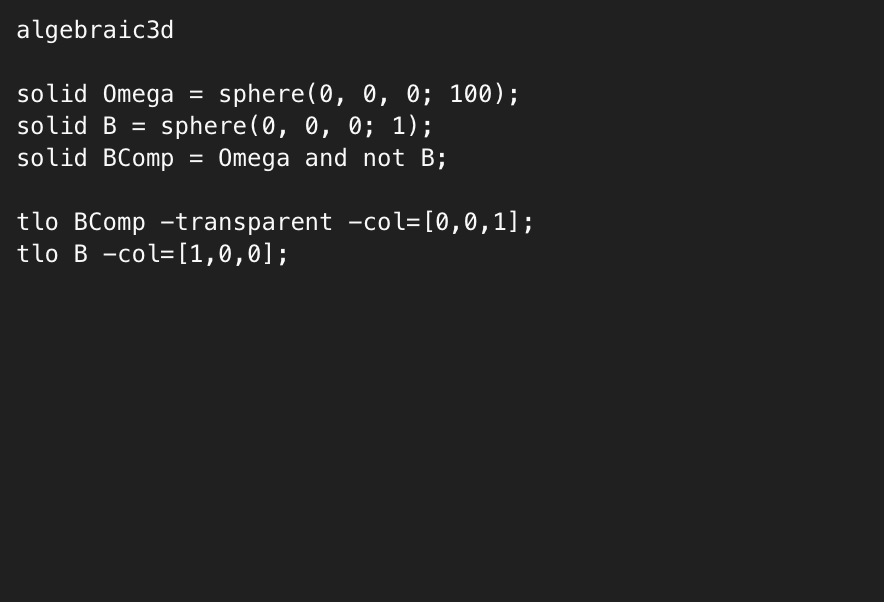
\includegraphics[width=0.48\textwidth, keepaspectratio]{Figures/ExampleSphere.png} & 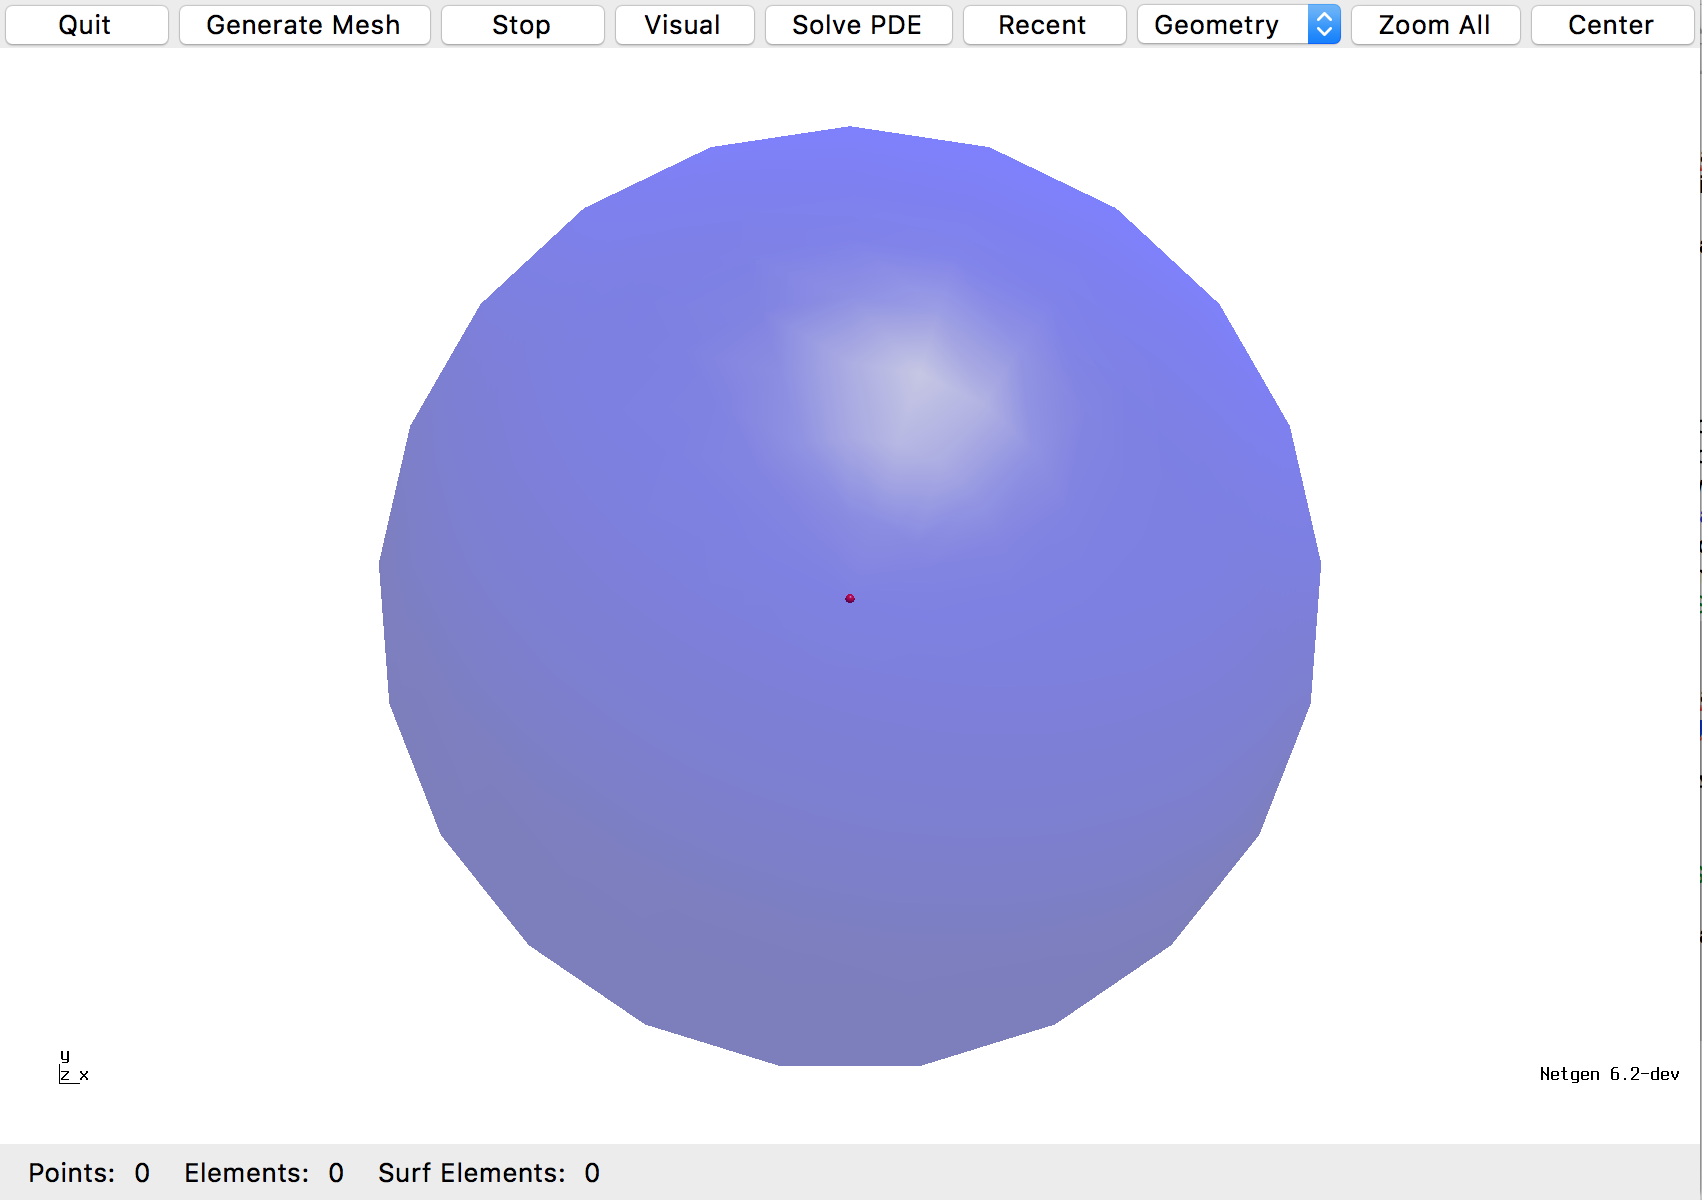
\includegraphics[width=0.48\textwidth, keepaspectratio]{Figures/ExampleSphereNetgen.png}\\
\textrm{\footnotesize{(a) Example of a \texttt{.geo} file describing a sphere in a sphere}} & \textrm{\footnotesize{(b) Visulisation of the \texttt{.geo} file in (a)}}
\end{array}$$
%\begin{figure}\label{LogvsLin}
\caption{Example of a \texttt{.geo} file (a) describing a sphere of unit radius contained in a domain consisting of a sphere with a radius of 100, with (b) a visualisation of of the constructed geometry using negten.}
\label{fig:ExampleSphere}
\end{figure}
\noindent
This example defines a unit sphere $B$ contained in a domain $\Omega$, which consists of a sphere with a radius of 100. Truncating the domain at a distance approximately 100 times the object size is sufficient for most cases. Next we discuss how to define the material properties of the different regions in the domain.
\subsection{Defining material properties}
To set the material parameters, the user is required to  label each region defined as a Top Level Object (tlo).  This is done by inserting a \texttt{\#} after each toplevel object followed by a label for the material, it's relative permeability $\mu_r$ and it's conductivity $\sigma_*$. We define the material properties for the example presented in the Section \ref{sectTruncating} in  the Figure \ref{fig:ExampleSphereMaterials}.

\begin{figure}[H]
\begin{center}
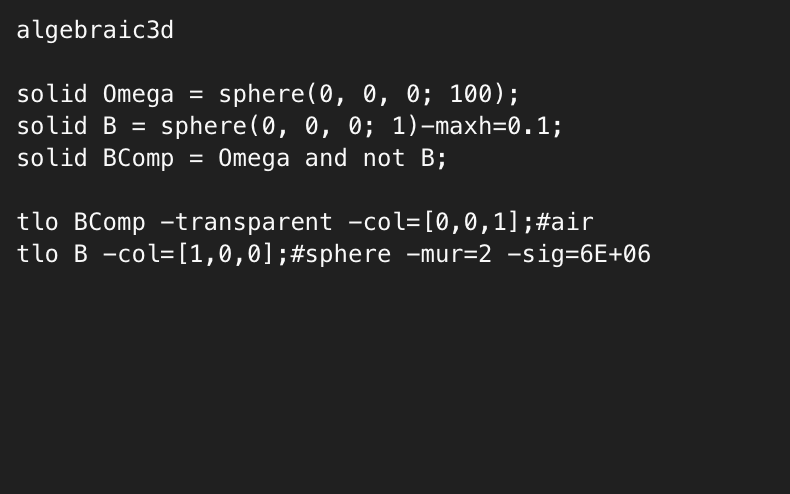
\includegraphics[width=0.5\textwidth]{Figures/ExampleSphereMaterials.png}
\caption{Image displaying an example of a \texttt{.geo} file with material properties defined for it's regions.}\label{fig:ExampleSphereMaterials}
\end{center}
\end{figure}
\noindent
In Figure \ref{fig:ExampleSphereMaterials}, \texttt{\#sphere -mur=2 -sig=6e+06} labels the object $B$ as \texttt{"sphere"} and defines it's material properties to be $\mu_r=2$ and $\sigma_*=6\times10^6 \text{S/m}$. The inclusion of \texttt{\#air} labels the non conducting region as \texttt{"air"}, which is a protected material and, therefore, does not require the user to input a value for $\mu_r$ or $\sigma_*$. Lastly,  note the inclusion of \texttt{-maxh=0.1} when defining the geometry of $B$. This is an inbuilt function of \texttt{Netgen} for meshing purposes allowing the user to specify a maximum element size for each region in the domain. This is useful since it allows the user to refine the mesh in the conducting region of the domain.\\
\\
Next, we specify the restrictions of the syntax for defining material properties. Any line which starts with \texttt{tlo} (which must have no spaces before) must also contain a material label defined as \texttt{\#material}. On the same line, the user must define both $\mu_r$ and $\sigma_*$ (unless the material is defined to be \texttt{\#air}), to do this the user must provide the flag \texttt{-mur=***} and \texttt{-sig=***} with at least one space between the two flags, but no spaces before or either of the equal signs, and with \texttt{***} replaced with value of the parameter. Note that  $\sigma_*$ should be specified in $\text{S/m}$. Some examples of this can be seen below, first the following examples are accepted,
\begin{align*}
&\texttt{tlo B -col=[1,0,0];\#sphere -mur=2 -sig=6E+06}\\
&\texttt{tlo B -col=[1,0,0];    $\quad$       \#sphere-mur=2 -sig=6E+06}\\
&\texttt{tlo B -col=[1,0,0];\#sphere   $\quad$    -mur=2   $\quad$  -sig=6E+06}
\end{align*}
However, the following examples will not work
\begin{align*}
&\texttt{tlo B -col=[1,0,0];\#sphere -mur = 2 -sig = 6E+06}\\
&\texttt{  tlo B -col=[1,0,0];\#sphere-mur=2 -sig=6E+06}\\
&\texttt{tlo B -col=[1,0,0];\#sphere -mur=2-sig=6E+06}\\
&\texttt{tlo B -col=[1,0,0];\#sphere}\\
&\texttt{-mur=2-sig=6E+06}
\end{align*}
Due to there being a space before or after the equal signs in the first; to a space before the \texttt{tlo} in the second; to the lack of a space between the definition of \texttt{-mur} and \texttt{-sig} in the third and due to the split two lines in the last.
\\
\\
We next consider the case of an object made up of multiple conducting regions follow the examples in Ledger, Lionheart and Amad~\cite{LedgerLionheartamad2019}. We define a conducting rectangular bar, $B$ which is a $2\times1\times1$ block made up 2 distinct sections, contained in a domain bounded by a sphere with radius of 100, as defined in the \texttt{.geo} file shown in Figure \ref{fig:DualBarExample}. Note that $B$ does not have units, the object $\alpha B$ has units with $\alpha$ being the size parameter specified in $\text{m}$ and $\alpha$ is specified later.

\begin{figure}[H]
\begin{center}
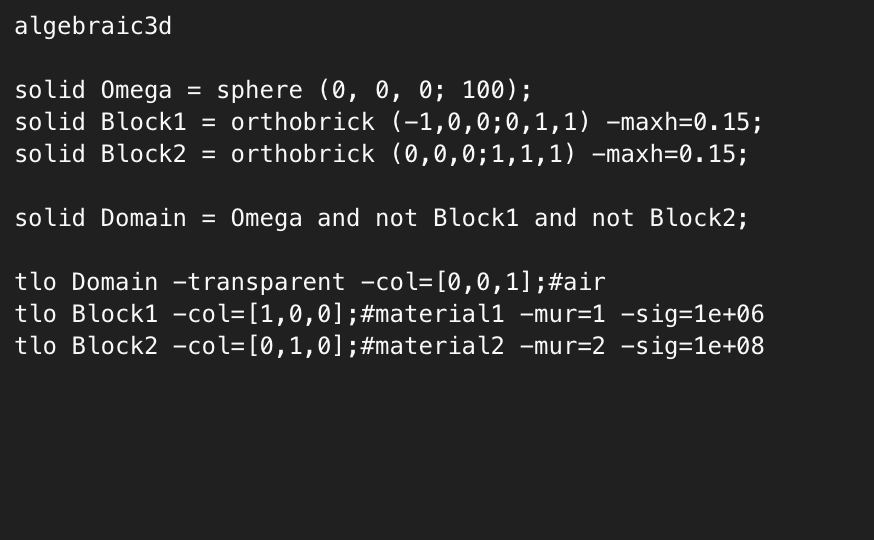
\includegraphics[width=0.5\textwidth]{Figures/DualBarExample.png}
\caption{Image displaying an example of a \texttt{.geo} file which defines a bar constructed of 2 regions with different material properties contained in a domain consisting of a sphere with a radius of 100.}\label{fig:DualBarExample}
\end{center}
\end{figure}
\noindent
In Figure \ref{fig:DualBarExample} we have defined two distinct regions \texttt{Block1} and \texttt{Block2} with materials \texttt{"Material1"} and \texttt{"Material2"} having different material properties, respectively.\\
\\
We finish this section with an example of two unit spheres which are constructed using the same material. An example of the \texttt{.geo} file can be seen in Figure \ref{fig:TwoSpheresExample}.

\begin{figure}[H]
\begin{center}
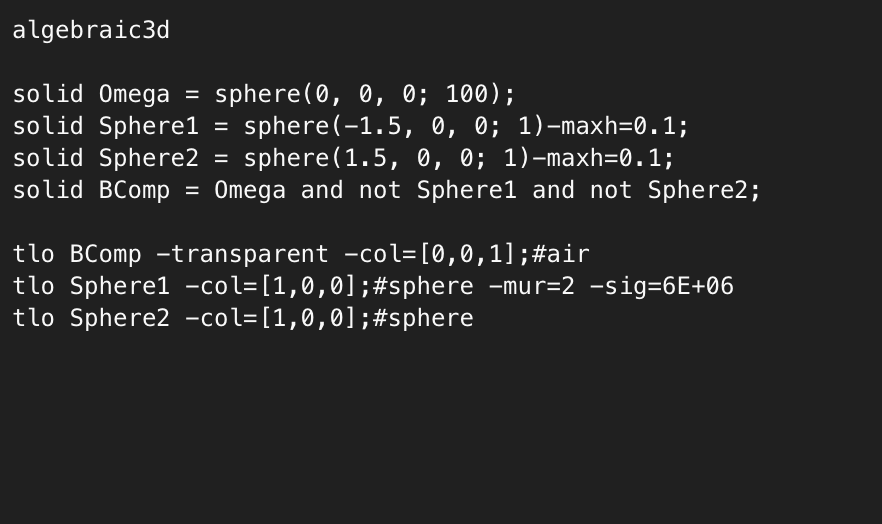
\includegraphics[width=0.5\textwidth]{Figures/TwoSpheresExample.png}
\caption{Image displaying an example of a \texttt{.geo} file which defines a bar constructed of 2 regions with different material properties contained in a domain consisting of a sphere with a radius of 100.}\label{fig:TwoSpheresExample}
\end{center}
\end{figure}
\noindent
This example demonstrates how we only need to define the material properties for \texttt{\#sphere} once even though there are two regions to which it will be applied. This makes it easier to change material properties for a whole geometry when made up of multiple \texttt{tlo}s. We expect this to be useful when working with more complex geometries such as that in the case of a rifle shell, which will be presented in Section \ref{sectRifle}.


\subsection{OCC Geometry}
The current version of \texttt{Netgen} (version 6.2.2203) supports defining object geometries via the Open Cascade Technology (OCC) format. Unlike the \texttt{.geo} file format, the OCC format is purely Python based. I.e. geometries are defined in \texttt{.py} files. Consequently, the user can use standard Python arguments and syntax. For example importing libraries and using iterative loops.\\

\noindent
In the same way as the \texttt{.geo} file format, \texttt{Netgen} constructs complex shapes out of simpler geometric primitives. Currently, \texttt{NGSolve} recommends that OCC geometries be used rather than \texttt{.𝚐𝚎𝚘} files, but there is little documentation available about available primitives and methods. For documentation, we refer the user to the \texttt{NGSolve} documentation and the Open Cascade Technology bottle example:, \href{https://docu.ngsolve.org/latest/i-tutorials/unit-4.4-occ/occ.html?highlight=occ}{here} and \href{https://dev.opencascade.org/doc/overview/html/occt__tutorial.html}{here}.\\

\noindent
An example OCC geometry file to define a unit radius sphere is presented in Listing \ref{lst:OCC_sphere}. In this example we illustrate introducing a unit radius sphere into a larger non-conducting truncated region. This example is included as \texttt{OCC\_Geometry/OCC\_sphere.py}.

\begin{lstlisting}[language=Python, caption={OCC description for a unit radius sphere inside a larger truncated non-conducting region.}, label={lst:OCC_sphere}]
from netgen.occ import *

# Setting mur, sigma, and defining the top level object name:
object_name = 'sphere'
mur = 1
sigma = 1e6

# setting radius
r = 1

# Generating OCC primative sphere centered at [0,0,0] with radius r:
sphere = Sphere(Pnt(0,0,0), r=r)

# Generating surrounding non-conducting region as [-1000,1000]^3 box:
box = Box(Pnt(-1000, -1000, -1000), Pnt(1000,1000,1000))

# setting material and bc names:
# For comparability, we want the non-conducting region to have the 'outer' boundary condition and be labelled as 'air'
sphere.mat(object_name)
sphere.bc('default')
box.mat('air')
box.bc('outer')

# Setting maxh:
sphere.maxh = 0.5
box.maxh = 1000

# Joining the two meshes:
# Glue joins two OCC objects together without interior elemements
joined_object = Glue([sphere, box])

# Generating Mesh:
geo = OCCGeometry(joined_object)
nmesh = geo.GenerateMesh()
nmesh.Save(r'VolFiles/OCC_sphere.vol')
\end{lstlisting}

Similarly to the \texttt{.geo} file format, we make specific mandates for the format. Each OCC geometry file must include:
\begin{lstlisting}[language=Python]
object_name = ['object 1', 'object 2', ... ]
sigma = [conductivity_1, conductivity_2, ...]
mur = [mur_1, mur_2, ...]
\end{lstlisting}
corresponding to the names (string) of the different sub-regions that make up the object and their conductivity (S/m) (float) and relative magnetic permeability (float) values respectively which, in the case of multiple sub-regions can be defined in the form of the lists. In the simplest case, where only one primitive is used, then these can be defined using a single entry. E.g.

\begin{lstlisting}[language=Python]
object_name = 'sphere'
sigma = 1e6
mur = 1
\end{lstlisting}
would define a single object called 'sphere' with conductivity $\sigma_*=10^6$ S/m and relative permeability $\mu_r = 1$.\\

\noindent
In addition, we also mandate that each mesh generated using the OCC format must be save using the same name as the \texttt{.py} file that defines the geometry. For example in Listing \ref{lst:OCC\_sphere}, we have the file name \texttt{OCC\_sphere.py} and save the generated mesh as \texttt{OCC\_sphere.vol}. In a similar way to the \texttt{.geo} file format, each OCC \texttt{.py} file must be stored in the \texttt{OCC\_Geometry} folder and each mesh must be stored in the \texttt{VolFiles} folder.\\

\noindent
Secondly, there must be a valid object description using the available OCC primitives and a defined non-conducting region. For example:
\begin{lstlisting}[language=Python]
sphere = Sphere(Pnt(0,0,0), r=1)
box = Box(Pnt(-1000,-1000,-1000), Pnt(1000,1000,1000))
\end{lstlisting}
defines a sphere of radius 1 and a large cube, centred at (0,0,0) with side length 2000. Note the similarities between the \texttt{.geo} file syntax for a simple primitive and the OCC primitive. We also need to specify material names, boundary condition names, and any additional properties (e.g. \texttt{𝚖𝚊𝚡𝚑}). For compatibility with \texttt{MPT-Calculator}, we want the non-conducting region to have the \texttt{'outer'} boundary condition and be labelled as \texttt{'air'}. In addition, the material name for the conducting object must match one of the entries in \texttt{object\_name}.

\begin{lstlisting}[language=Python]
sphere.mat(object_name[0])
sphere.bc('default')
box.mat('air')
box.bc('outer')
\end{lstlisting}

\noindent
Finally, we need to join the non-conducting region with the conducting object. To avoid interior elements, we use the \texttt{𝙶𝚕𝚞𝚎} method:
\begin{lstlisting}[language=Python]
joined_object = Glue([sphere, box])
\end{lstlisting}
Once the geometric description has been defined, the user must generate and save a mesh. This is done using the \texttt{OCCGeometry}, \texttt{GenerateMesh}, and \texttt{Save} methods. E.g.
\begin{lstlisting}[language=Python]
geo = OCCGeometry(joined_object)
nmesh = geo.GenerateMesh()
nmesh.Save(r'VolFiles/OCC_sphere.vol')
\end{lstlisting}
We recommend that the user maintains a similar style when defining OCC \texttt{.py} files to ensure compatibility. In addition, \texttt{GenerateMesh} admits multiple meshing arguments, such as \texttt{meshsize.very\_coarse}, \texttt{meshsize.coarse}, \texttt{meshsize.moderate}, ect that have the same effect as the mesh size options discussed in Section~\ref{sectmain.py}.\\

\noindent
Further examples are provided in the \texttt{OCC\_Geometry} folder.
